%\documentclass[aps,prd,nofootinbib,amsmath,notitlepage]{revtex4-1}
\documentclass[11pt]{article}
\usepackage{jcappub,graphicx,array,multirow,dcolumn,hyperref,bm,pbox,color,verbatim, slashed}
\usepackage[T1]{fontenc}
\usepackage[usenames]{xcolor}
\usepackage[section]{placeins} % Keep floats within the relevant section
\usepackage[final]{pdfpages}
\DeclareMathOperator{\ev}{eV} \DeclareMathOperator{\kev}{KeV} \DeclareMathOperator{\mev}{MeV} \DeclareMathOperator{\gev}{GeV} \DeclareMathOperator{\tev}{TeV} \DeclareMathOperator{\cm}{cm} \DeclareMathOperator{\barn}{barn} \DeclareMathOperator{\g}{g} \DeclareMathOperator{\km}{km} \DeclareMathOperator{\pb}{pb} \DeclareMathOperator{\s}{s} \DeclareMathOperator{\yr}{yr}\DeclareMathOperator{\gyr}{Gyr} \DeclareMathOperator{\kg}{kg} \DeclareMathOperator{\mpc}{Mpc} \DeclareMathOperator{\few}{few} \DeclareMathOperator{\kel}{K}
\newcommand{\cA}{{\cal A}} \newcommand{\cC}{{\cal C}} \newcommand{\cD}{{\cal D}} \newcommand{\cE}{{\cal E}} \newcommand{\cF}{{ \cal F}} \newcommand{\cH}{{\cal H}} \newcommand{\cJ}{{\cal J}} \newcommand{\cL}{{\cal L}} \newcommand{\cM}{{\cal M}} \newcommand{\cN}{{\cal N}} \newcommand{\cO}{{\cal O}} \newcommand{\cP}{{ \cal P}} \newcommand{\tp}{{ \tilde p}} \newcommand{\cR}{{\cal R}} \newcommand{\cS}{{\cal S}}
\newcommand{\ep}{\epsilon} \newcommand{\vp}{\varphi} \newcommand{\half}{\frac12}
\newcommand{\ie}{{\it i.e.~}}  \newcommand{\eg}{{\it e.g.~}}
\newcommand{\pt}{\partial} \def\d{{\rm d}}  \def\oL{\overline} \def\wh{\widehat}
\newcommand{\pL}{\left(} \newcommand{\pR}{\right)} \newcommand{\bL}{\left[} \newcommand{\bR}{\right]} \newcommand{\cbL}{\left\{} \newcommand{\cbR}{\right\}} \newcommand{\mL}{\left|} \newcommand{\mR}{\right|}
\newcommand{\beq}{\begin{equation}} \newcommand{\eeq}{\end{equation}}
\newcommand{\bea}{\begin{eqnarray}} \newcommand{\eea}{\end{eqnarray}}
\newcommand{\alg}[1]{\begin{align} \begin{split} #1 \end{split}  \end{align}}
\newcommand{\vev}[1]{\langle {#1} \rangle}
\newcommand{\tenx}[1]{\times 10^{#1}}
\newcommand{\Eq}[1]{Eq.~(\ref{#1})} \newcommand{\Eqs}[2]{Eqs.~(\ref{#1}) and (\ref{#2})} \newcommand{\Eqm}[2]{Eqs.~(\ref{#1}) through (\ref{#2})}
\newcommand{\Sec}[1]{Sec.~\ref{#1}} \newcommand{\Secs}[2]{Secs.~\ref{#1} and \ref{#2}} \newcommand{\Secm}[2]{Secs.~\ref{#1} through \ref{#2}}
\newcommand{\Fig}[1]{Fig.~\ref{#1}} \newcommand{\Figs}[2]{Figs.~\ref{#1} and \ref{#2}}
\newcommand{\Tab}[1]{Tab.~\ref{#1}}
\newcommand{\App}[1]{App.~\ref{#1}}
\DeclareMathOperator{\br}{Br} \DeclareMathOperator{\tr}{Tr}
%%%%% Particle Physics %%%%%
\def\lag{\mathcal{L}}
\def\lagint{\lag_\text{int}}
\def\op{\mathcal{O}}
\def\oprel{\mathcal{O}^\text{rel}}
\def\chibar{\bar{\chi}}
\def\Nbar{\bar{N}}
%%%%% Nuclear Response Function, quantities %%%%%
\def\W{\widetilde{W}}
%% for consistency with particle physics literature, don't use bold face
\def\sp{\langle {S}_p \rangle }
\def\sn{\langle {S}_n \rangle }
\def\sN{\langle {S}_N \rangle }
\def\Lp{\langle {L}_p \rangle }
\def\Ln{\langle {L}_n \rangle }
\def\LN{\langle {L}_N \rangle }
%%%%% momentum short-hand %%%%%
\def\qsq{\vec{q}^{\,2}}
\def\absq{|\vec{q}|}
\def\qbar{\bar{q}}
\def\vqsq{\vec{q}^{\,2}}
\def\mag{\tilde{\mu}}
\newcommand{\arxiv}[1]{{\href{http://arxiv.org/abs/#1}{\tt #1}}}

\newcommand{\sdm}[1]{\textcolor{blue}{\textbf{(#1 -- SDM)}}}


\begin{document}
\title{Model Selection with a Single Target:\\Leveraging Annual Modulation to Differentiate Direct Detection Signals}
\author{Samuel J.~Witte${}^a$,}
\affiliation[a]{\dots}
\author{Vera Gluscevic${}^b$, and}
\affiliation[b]{\dots}
\author{Samuel D.~McDermott${}^c$}
\affiliation[c]{C.~N.~Yang Institute for Theoretical Physics, Stony Brook, NY, USA}\subheader{\rm YITP-SB-16-NN}


\abstract{
\sdm{I've listed the authors as if this is an astro-ph paper, but perhaps it will be more suitable for hep-ph, and should be alphabetical? No need to decide immediately.} Abstract goes here, and it will say lots of interesting stuff when we finally figure out our conclusions, but for now this is just a placeholder. Abstract goes here, and it will say lots of interesting stuff when we finally figure out our conclusions, but for now this is just a placeholder. Abstract goes here, and it will say lots of interesting stuff when we finally figure out our conclusions, but for now this is just a placeholder. Abstract goes here, and it will say lots of interesting stuff when we finally figure out our conclusions, but for now this is just a placeholder.
}

\maketitle

\section{Introduction} \setcounter{page}{2}

Experimental evidence from a vast array of independent sources conclusively demonstrates the existence of a non-baryonic form of matter in the universe. This so-called dark matter is the dominant source of the gravitational potential wells that have determined the large scale structure of the universe, but dark matter particles have yet to be observed in a laboratory setting. Despite an experimental direct detection program that has now been mature for several decades, all evidence in favor of the existence of dark matter is instead furnished by indirect observations of cosmological and astrophysical settings.

There are good reasons to be optimistic that direct detection may be on the cusp of important discoveries, however. As next-generation experiments that incorporate increasingly precise detection technologies come online, we will be pushing through the final parameter space before encountering the astrophysical neutrino background. Luckily, many interesting theories of dark matter predict scattering cross sections in this range. For example, heavy $SU(2)$-doublet and -triplet fermions, such as the Higgsinos and the wino of supersymmetry, are expected to have cross sections of order $\sigma_{\rm SI} \sim \cO(\few\tenx{-48})\cm^2$, fixed by their Standard Model gauge quantum numbers alone \cite{Hill:2011be,Hill:2013hoa,Hill:2014yxa}, while a heavy $SU(2)$-singlet fermion, like the bino, is around an order of magnitude lower depending on its coannihilation partner \cite{Berlin:2015njh}. Models with kinematically suppressed tree-level scattering may also be embedded in more complete dark sectors that have loop-level cross sections in this same range \cite{Ipek:2014gua,McDermott:2014rqa,Appelquist:2015yfa,Appelquist:2015zfa}.

Because so many theories can be accommodated in the parameter space that we will imminently probe, we must plan for the science opportunities associated with the first detection of dark matter particles. The ``inverse problem'' that we will confront upon successful detection of dark matter particles is that of understanding the (high-energy) dark sector dynamics solely by examining (low-energy) recoils of detector elements. In collider physics terms, the luminosity is fixed by the dark matter astrophysics, making measurements of dark matter properties possible only at a single energy scale. We will need to reconstruct the interesting physics of the dark sector at all scales from nuclear recoils alone, despite the fact that the details of the dynamics that link the dark sector to the Standard Model are most likely integrated well above the low energies probed in direct detection experiments. On the other hand, because the dynamics are coarse grained at the energies of direct detection experiments, the nuclear responses are compactly described by an easily exhaustible list of interactions. These are collected as a nonrelativistic effective field theory \cite{Fitzpatrick:2012ix, Anand:2013yka}. This ``effective field theory of dark matter direct detection'' reproduces the nontrivial nuclear physics induced by some of the best-motivated UV-complete theories of dark matter \cite{Gresham:2014vja, Gluscevic:2015sqa}. %As described presently, we can look for clues to the nature of the dark sector along two orthogonal axes with the help of this effective theory.
All of the characteristic information about the dark sector interactions is contained in the coefficients of the effective theory. The key to accessing this information and unlocking the secrets of the dark matter interactions lies in the careful study of the scattering data in the event of a detection.

Much of the information one might hope to access from a direct detection experiment is contained in the energy spectra of nuclear or electronic recoils. Due to Poisson noise and degeneracies in the spectra of different interactions, model selection using spectral information alone is difficult with a single target material. However, recent studies show it is possible to discriminate between interactions by leveraging the energy spectra from nuclei with sufficiently diverse nuclear physics characteristics. Thus, energy spectra of experiments with different nuclei can break degeneracies in the dark matter model space, as long as the target nuclei have ``complementary'' nuclear physics characteristics \cite{McDermott:2011hx,Peter:2013aha,Gluscevic:2014vga,Catena:2014epa,Catena:2014hla,Dent:2015zpa,Gluscevic:2015sqa}.

In this work, we will be interested in a different route to the dynamics of the dark sector from low-energy physics: we will show that information from the time distribution of scattering events also helps break degeneracies in model space. Almost since the dawn of the study of direct detection experiments, the annual modulation of the direct detection rate \cite{Freese:1987wu} has been appreciated to provide a distinctive dark matter signature, as have its higher harmonics \cite{Freese:2012xd,Lee:2013xxa} and the disturbance of its phase space from nonstandard astrophysics \cite{Green:2000ga,Gelmini:2000dm} as well as from the influence the solar system gravitational field \cite{Lee:2013wza,DelNobile:2015tza,DelNobile:2015nua,DelNobile:2015rmp}. Later, it was pointed out that similar effects are produced from nonstandard particle physics models \cite{DelNobile:2015tza}. Here we will demonstrate that even within classes of interactions with approximately degenerate recoil spectra the additional discrimination power from timing information will allow some of the most popular detector designs to go beyond detection and actually achieve comprehensive {\it model selection}. \sdm{in the G2 experiments? G3? before the neutrino floor? never? just shooting from the hip here. We will say more as we actually get conclusions}. In this way, it may be possible to discriminate between certain models of the dark matter using a single detector element on its own.

The rest of the paper is laid out like \sdm{every other good paper you've read, and totally unlike all the bad papers that you usually read}.




\section{Dark Matter Direct Detection: Energy and Time Dependence}

The observed recoil energy spectrum is the number count of nuclear recoil events observed per recoil energy $E_R$, per unit time, per unit target mass,
\begin{equation}
\frac{dR}{dE_R dt}(E_R,t) =  \frac{\rho_\chi}{m_T m_\chi} \int\limits_{v_{\mathrm{min}}}^{v_{\mathrm{esc, lab}}}  v f(\mathrm{\mbox{\bf{v}}}|t) \frac{d\sigma_T}{dE_R} (E_R,v) d^3v ,
\label{eq:dRdEr_general}
\end{equation}
where:
\begin{itemize}
\item $\rho_\chi$ and $m_\chi$ are the local dark matter density and the dark matter particle mass
\item $v_\mathrm{min} = \sqrt{m_T E_R/2\mu_T^2}$ is the minimum velocity a dark matter particle of mass $m_\chi$ needs to produce a nuclear recoil of energy $E_R$, where $\mu_T=\frac{m_Tm_\chi}{m_T+m_\chi}$ is the reduced mass of the dark matter particle and the target nucleus
\item $v_{\mathrm{esc, lab}}$ is the escape velocity from the Galactic halo in the lab frame
\item $v$ is the velocity of the dark matter in the lab frame
\item $f(\mathrm{\mbox{\bf{v}}}|t)$ is the observed dark matter velocity distribution, which is generically time-dependent
\item and $d\sigma_T/dE_R=m_T \sigma_T /2\mu_T^2 v^2$ is the differential cross section for dark matter scattering off a target; in this work, we focus on nuclear recoils, and we focus on the physics of $d\sigma_T/dE_R=m_T \sigma_T /2\mu_T^2 v^2$ in the next section.
\end{itemize}
The differential rate in \Eq{eq:dRdEr_general} is determined by the experimental setup, the dark matter astrophysics, the particle properties of dark matter, the nuclear properties of the target material $T$ (throughout this paper we use $T$ to denote the nuclear target and we reserve $N$ to denote a nucleon, either $n$ or $p$), and the type of interaction between the dark matter and the target. For the purposes of this study, we set the astrophysical parameters to the following values \cite{Bovy:2013raa}: $\rho_\chi=0.3$ GeV/cm$^3$; $v_{\mathrm{esc}} = 544$ km/sec in the Galactic frame; we assume that $f(\mathrm{\mbox{\bf{v}}})$ is a Maxwellian distribution in the Galactic frame, with an rms speed of $155$ km/sec, and a mean speed equal to the Sun's rotational velocity around the Galactic center, $v_\textrm{lag}=220$ km/sec. The underlying particle physics model determines the calculation of the recoil rate through the differential scattering cross section ${d\sigma_T}/{dE_R}$, as discussed in \cite{Gluscevic:2015sqa,Gresham:2014vja}: this has a free normalization with units of cm${}^2$ as well as a discrete set of functional dependences on $E_R$ and $v$.

The total rate $R$ of events is the integral of the differential rate within the nuclear-recoil energy range $\cE$ of a given experiment\footnote{For simplicity, in this work we assume unit efficiency of detection, at all energies within the analysis window, for each experiment considered here, and rescale the exposures to take this assumption into account when choosing experimental parameters to represent the capabilities of G2 experiments.}, $R(t)=\int_\cE \frac{dR}{dE_R dt} dE_R$. In turn, the total expected number of events $N$ for a target of total mass $\cM$ from a time $t_1$ to $t_2$ over the range $\cE$ is
\beq
N =  \cM \int\limits_{t_1}^{t_2} \int\limits_\cE  \frac{dR}{dE_R dt}(E_R,t)\,dE_R \,dt.
\eeq
The total number of events and the differential rate for a given energy and time will be used to define a likelihood function. This likelihood can be interpreted as a function of particle physics inputs, which in turn parameterize a posterior probability distribution. The integral over this posterior will finally provide a Bayesian evidence in favor of a particular model. Comparing evidence from different particle physics models allows model selection as described in \cite{Gluscevic:2014vga, Gluscevic:2015sqa}.

As is clear in \Eq{eq:dRdEr_general}, the differential rate of nuclear recoils depends on time. This arises from the motion of the earth about the sun. In the galactic rest frame, the dark matter is well approximated as a virialized fluid with a Maxwell-Boltzmann velocity distribution whose most probable speed is a function of radius. However, a terrestrial laboratory experiences additional motion relative to such a reference frame. The consequence of this motion is that on earth we appear to be moving harmonically with respect to a galactic ``wind'' of dark matter particles. In prior work this harmonic motion was effectively averaged over, such that time information was simply accounted for as an overall scaling of the total exposure. Here, instead of integrating over the time we instead examine what it tells us about the underlying interaction.




\section{Effective Field Theory and Dark Matter Scattering}

The function $d\sigma_T/dE_R=m_T \sigma_T /2\mu_T^2 v^2$ defined above contains the interesting particle physics of the dark matter scattering. In this section, we discuss that this scattering can take only a limited number of forms which are catalogued by an effective field theory. We highlight several particularly interesting examples of this scattering, which we will subsequently use to test the effects of time dependence on model selection.

\subsection{Momentum and Velocity Suppression: Scaling in Energy and Time}

Spin-independent scattering involves coherent contributions from an entire nucleus, such that the cross section scales quadratically with nucleon number. This is to be contrasted with the spin-dependent rate, since the total nuclear spin is typically concentrated in a single nucleon and does not scale with nuclear size. However, ``spin-independent'' only refers to the dependence on nuclear spin and need not imply a large rate. Many responses sensitive to a several nuclear ``charges'' and ``currents'' \cite{Fitzpatrick:2012ix}, some of which are suppressed by small kinematic factors, can be classified as ``spin-independent.'' Consistently counting the pertinent small factors requires a proper effective field theory expansion. The effective field theory of dark matter direct detection \cite{Fitzpatrick:2012ix, Anand:2013yka} is an expansion in two small kinematic variables: $|\vec q|/m_N$, where $\vec q$ is the change in momentum of the dark matter particle during the scattering, and $v_\perp$, the (orthogonal component of the) relative velocity of the initial state particles. For an incoming (outgoing) dark matter three-momentum $\vec p(\vec p')$, incoming (outgoing) target three-momentum $\vec k(\vec k')$, and reduced mass $\mu_{\chi N} = m_\chi m_N/(m_\chi +m_N)$, we define these kinematic factors as \cite{Fitzpatrick:2012ix}
\beq \label{eq:kinematic-definitions}
\vec q=\vec p'-\vec p=\vec k-\vec k', \qquad v_\perp=\frac{\vec p}{m_\chi}-\frac{\vec k}{m_N}+\frac{\vec q}{2\mu_{\chi N}}.
\eeq
The three momentum is directly related to the nuclear recoil energy $E_R$ via $\qsq=2m_TE_R$.

These expansion parameters are of the same order of magnitude, but they manifest differently in the observables of the scattering. In particular, responses that enter at higher order in $|\vec q|/m_N$ deliver a vanishing rate at both small and large momentum transfer, with a maximum rate at some intermediate recoil energy. On the other hand, higher order terms in $v_\perp$ monotonically decrease with energy, qualitatively similar to standard scattering. The novelty of the responses with $v_\perp$ dependence, therefore, is not easy to assess given a single energy spectrum. One solution is to leverage ``target complementarity'' by using a different nucleus with incommensurate nuclear charges \cite{Gluscevic:2015sqa}. We take a different approach here, starting from the observation that rates with a response proportional to $v_\perp^2$ include a nonstandard velocity integral in \Eq{eq:dRdEr_general}, leading to a novel dependence on laboratory velocity (as well as the astrophysical parameters) in the differential rate \cite{Fitzpatrick:2010br}. Because the laboratory velocity is changing with time, the different dependence on this velocity implicitly leads to a nonstandard time dependence for the interactions whose scattering cross sections include a factor of $v_\perp^2$. For large enough dark matter mass, this nonstandard time dependence can provide the {\it opposite phase} compared to the standard rate! Thus, a new observable can reveal the novelty of the responses with $v_\perp$ dependence: we can use phase information from rates with nonstandard velocity integrals to distinguish these from the standard rates.

%Distinguishing between rates with different momentum dependence is easy to do even when limiting to energy spectrum information from a single detector target element \cite{Gluscevic:2015sqa}. However, extracting the particle physics from two rates with the same momentum dependence requires additional information. This is true because interactions with different momentum dependence have qualitatively different energy spectra, whereas those with the same momentum dependence (even if the $v_\perp$ dependence differs) have energy spectra whose differences can be swamped by Poisson noise. The additional power needed for positive model selection can come from simultaneously examining spectra from detectors with complementary nuclear physics properties \cite{Gluscevic:2015sqa}. Alternately, a different route to this model discrimination is provided by the different time dependence noted here.

As an example, we show in \Fig{} how the different momentum and velocity dependences enter the energy and time spectra for different operators. \sdm{Here I think we should show one plot of $dR/dE_R dt$ vs $E_R$ spectrum for regular SI, ED-heavy, and anapole (taken on the equinox, for example); then another plot with the same interactions but $dR/dE_R dt$ vs $t$ for some reasonable energy deposition well above threshold. Use Xe detector \& 500 GeV particle, or whatever looks best} The energy spectra for the SI and ED-heavy interactions are visually distinguishable in a way that the SI and anapole interactions are not: it does not take an arbitrarily large exposure to collect a sufficient number of events to distinguish between the SI and ED-heavy hypotheses using the energy spectrum alone, although doing the same with the SI and anapole hypotheses is quite challenging, given realistic Poisson errors \cite{Gluscevic:2015sqa}. However, as a function of time it is clear that the anapole and SI rates have different phases as functions of time. This difference, expected to be a few percent given standard calculations for the modulation power fraction, is not sufficiently powerful on its own to differentiate two models with similar energy spectra. Nonetheless, we will show below that this small effect can be leveraged to supplement the energy spectrum information to allow for successful model selection with a smaller number of total events than would be required using energy spectrum information alone.

\subsection{Summary of Models}

With this physics motivation in mind, we examine the ability to perform model selection on models of new physics with a heavy gauge boson of mass $M$ that kinetically mixes with the Standard Model photon. At high energies, the Lagrangian contains
\beq \label{eq:UV-model}
\cL \supset -  m_X \bar X X + i \bar X \slashed D X  - \frac12 M^2 A'_\mu A'^\mu  - \frac14 F'_{\mu \nu} F'^{\mu \nu} - \frac\epsilon2 F'_{\mu \nu} F^{\mu \nu}
\eeq
for a fermion (or family of fermions, or charged supermultiplet) $X$ charged under a $U(1)'$ with vector $A'_\mu$ and gauge boson field strength $F'_{\mu \nu}$. At low energies, the dark matter couples to the Standard Model nucleon current \cite{Gresham:2014vja},
\beq \label{eq:current}
\cJ_\mu = \partial^\alpha F_{\alpha \mu} = e \sum_{n,p} \bar N \pL Q_N \frac{K_\mu}{2m_N} -\widetilde \mu_N \frac{i \sigma_{\mu \nu}q^\nu}{2m_N} \pR N,
\eeq 
where $Q_{p(n)}=1(0)$ are the nucleon charges in units of the electron charge $e$, $K_\mu/2 = (k_\mu + k'_\mu)/2$ is the average nucleon momentum, and $\tilde{\mu}_N = {\text{magnetic moment} \over \text{nuclear magneton}}$ is the dimensionless nucleon magnetic moment. At low energies, the model in \Eq{eq:UV-model} can give rise to several electromagnetic currents. These are determined by the charges and low-energy dynamics of the fermion dark matter particle, with candidate operators \cite{Gresham:2014vja, Gluscevic:2015sqa}
\begin{eqnarray} \label{eq:photon-DM-ops}
\cO_{\rm \chi, Anapole}^\mu & = & g^{\rm Anapole}\bar \chi \gamma^\mu \gamma_5 \chi, \\
\cO_{\rm \chi, MD}^\mu & = & \frac{g^{\rm MD}}{\Lambda}\bar \chi i \sigma^{\mu \nu} q_\nu \chi ,\\
\cO_{\rm \chi, ED}^\mu & = & \frac{g^{\rm ED}}{\Lambda} \bar \chi i \sigma^{\mu \nu} \gamma_5 q_\nu \chi.
\end{eqnarray}
The correct interaction operator for the low-energy interacting state $\chi$ is determined by the dynamics of the $X$ fermion(s) introduced above. The anapole current in \Eq{eq:photon-DM-ops} can arise if charged $X$ states condense to form a neutral Majorana state $\chi$ \cite{Bagnasco:1993st}, or the dipole currents form if an electromagnetically neutral $X^0$ couples to an electromagnetically charged pair of partner $X^\pm$ particles (of appropriate spin) \cite{Weiner:2012gm}. The scale at which the charged $X$ states are integrated out is $\Lambda$.

The simplicity of the model building notwithstanding, a rich assortment of momentum and velocity dependence appears in the EFT responses. We list the EFT classification of these operators in \Tab{tab:operators}. (This is an abbreviated version of the more exhaustive table that appeared in \cite{Gluscevic:2015sqa}, using results of \cite{Gresham:2014vja, Gluscevic:2015sqa}.% For additional details of the implementation of the effective theory in the context of model selection, we refer to the discussion in \cite{Gluscevic:2015sqa}.
)



\begin{table}[tb]
\begin{centering}
\renewcommand{\arraystretch}{1.3}
\begin{tabular}{c |>{$}c<{$}| >{$}c<{$} >{$}c<{$} c } \hline
 Model name & {\rm Lagrangian} & \text{$\vec q$, $v$ Dependence} &  {\rm Response}  
\\ \hline 
 SI & \frac g{M^2}\bar \chi \chi \bar N N & 1 & M
\\ \hline 
 \multirow{2}{*}{Anapole} & \multirow{2}{*}{$\frac g{M^2}\chibar \gamma^\mu \gamma_5 \chi \, \cJ_\mu $} & v_\perp^2 & M \\  
 & & \qsq/m_N^2 & \Delta + \Sigma' 
\\ \hline
\multirow{2}{*}{\pbox{20cm}{Magnetic Dipole}} & \multirow{2}{*}{$\frac g{\Lambda M^2} \chibar \sigma^{\mu \nu} \chi  \, q_\nu \cJ_\mu $} & \frac{\vec q^{\,4}}{\Lambda^4}+ \frac{\qsq v_\perp^2 }{\Lambda^2} & M \\
 & & \vec q^{\,4}/\Lambda^4 & \Delta + \Sigma' 
\\ \hline
Electric Dipole & \frac g{\Lambda M^2} \chibar \sigma^{\mu \nu} \gamma_5 \chi \, q_\nu \cJ_\mu  & \qsq /\Lambda^2 & M 
\\ \hline 
\end{tabular}
\caption{Selection of operators along with their EFT dependences, adapted from \cite{Gluscevic:2015sqa}. For the dipole models, we assume the mediator mass is large compared to the characteristic momentum transfer. The nucleon electromagnetic current $\cJ_\mu$ is defined in \Eq{eq:current}; the transverse velocity $v_\perp$ and three--momentum transfer $\vec q$ are defined in terms of the collision momenta in \Eq{eq:kinematic-definitions}; and $\Lambda$ is a heavy mass or compositeness scale appearing in the dipole models. The parametric momentum and velocity dependences (third column) schematically multiply the adjacent EFT response (fourth column).}
\label{tab:operators} 
\end{centering}
\end{table}



\section{Model Selection}

We perform Bayesian model selection, ...

\subsection{Simulations}

We simulate the following experimental set ups...

\subsection{Data Analysis}

\begin{figure*}
\centering
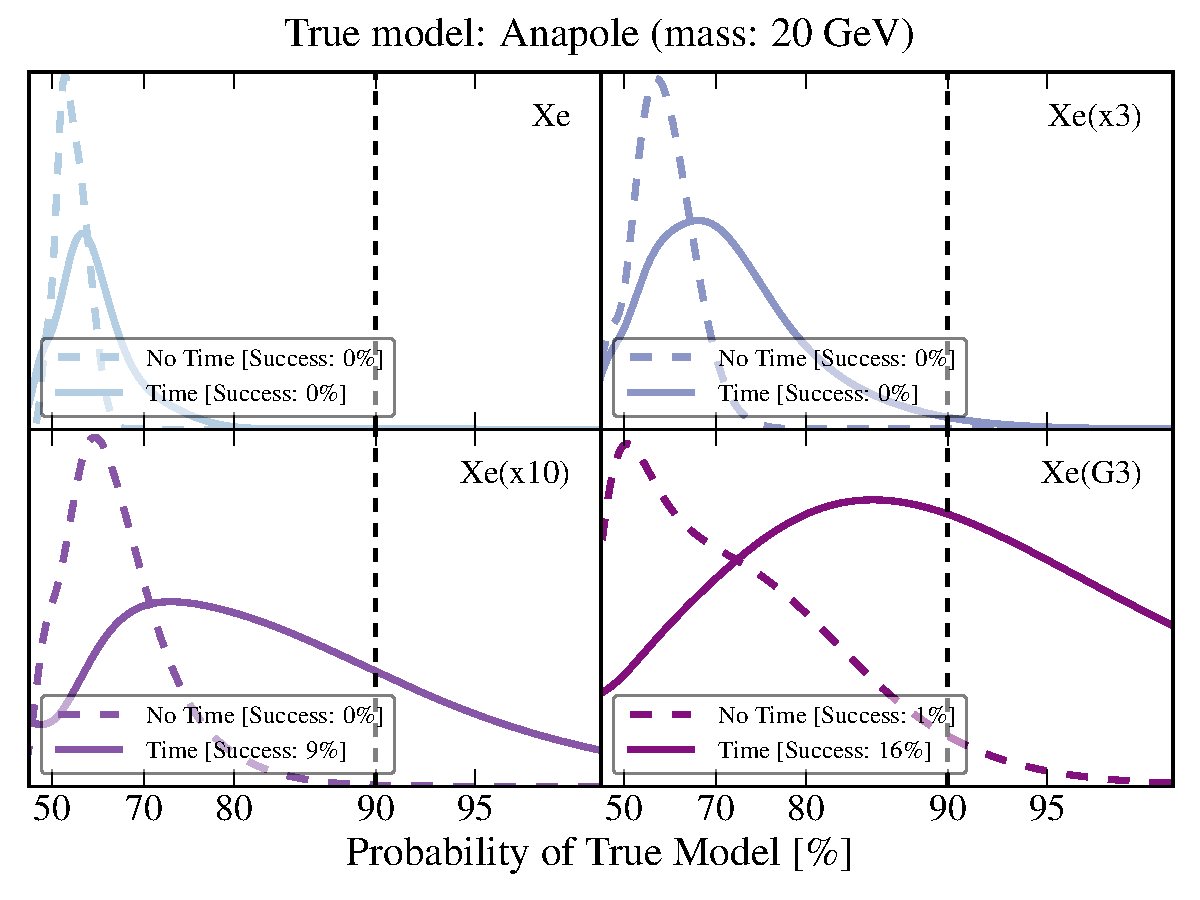
\includegraphics[width=0.7\textwidth]{plots/PDF_20GeV_Anapole_50sims_Xe_Xe3x_Xe10x_XeG3_GF_TNT.pdf}
\caption{\label{fig:500gev_anapole_XeFull_TNT_GF}}
\end{figure*}

\begin{figure*}
\centering
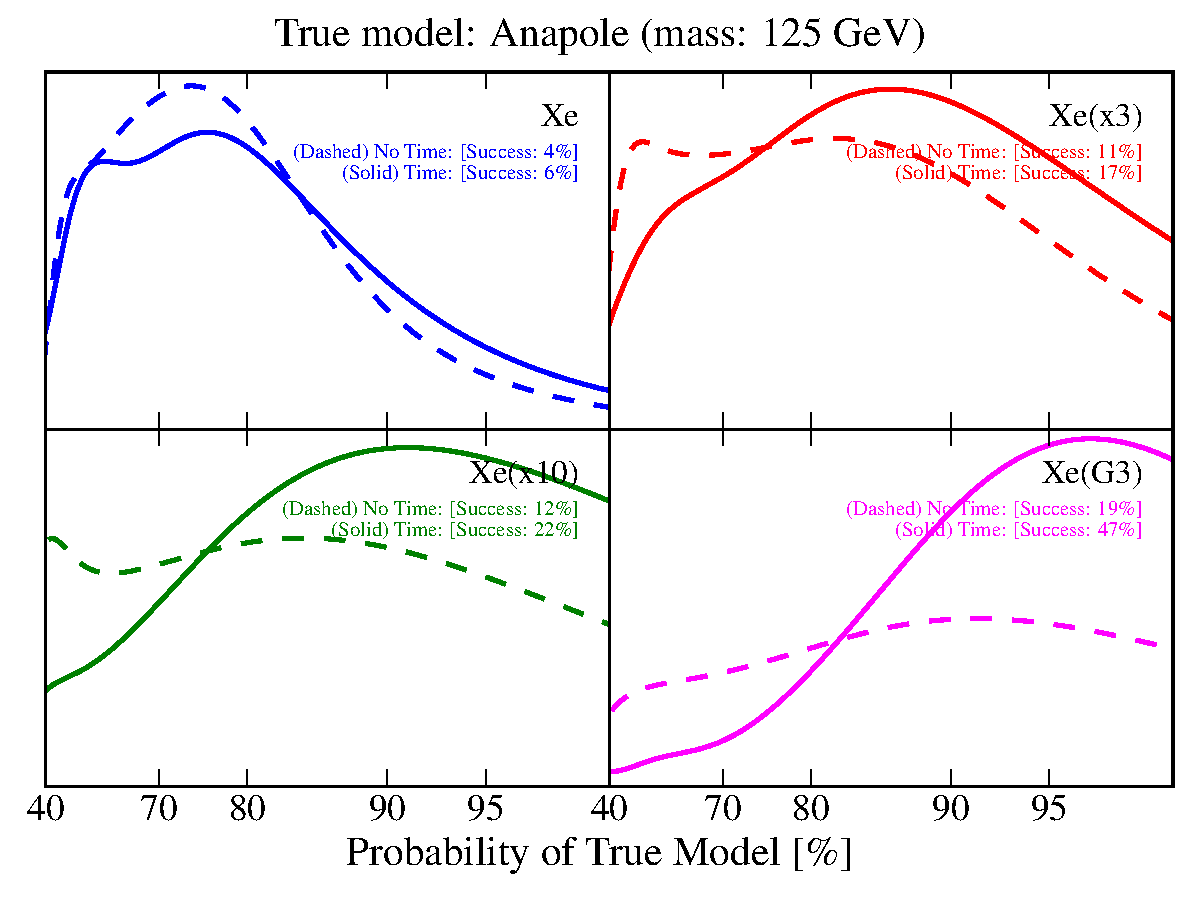
\includegraphics[width=0.7\textwidth]{plots/PDF_125GeV_Anapole_50sims_Xe_Xe3x_Xe10x_XeG3_GF_TNT.pdf}
\caption{\label{fig:500gev_anapole_XeFull_TNT_GF}}
\end{figure*}

\begin{figure*}
\centering
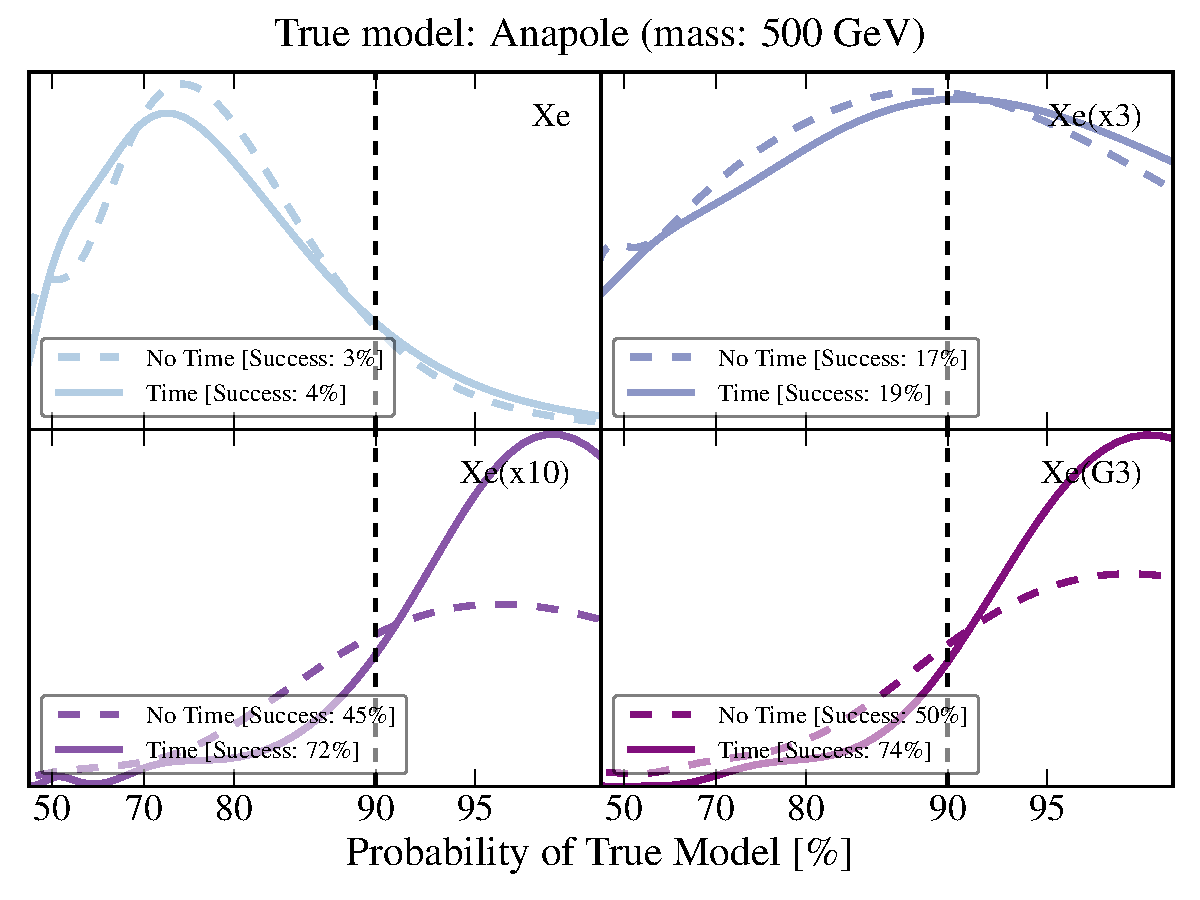
\includegraphics[width=0.7\textwidth]{plots/PDF_500GeV_Anapole_50sims_Xe_Xe3x_Xe10x_XeG3_GF_TNT.pdf}
\caption{\label{fig:500gev_anapole_XeFull_TNT_GF}}
\end{figure*}

\begin{figure*}
\centering
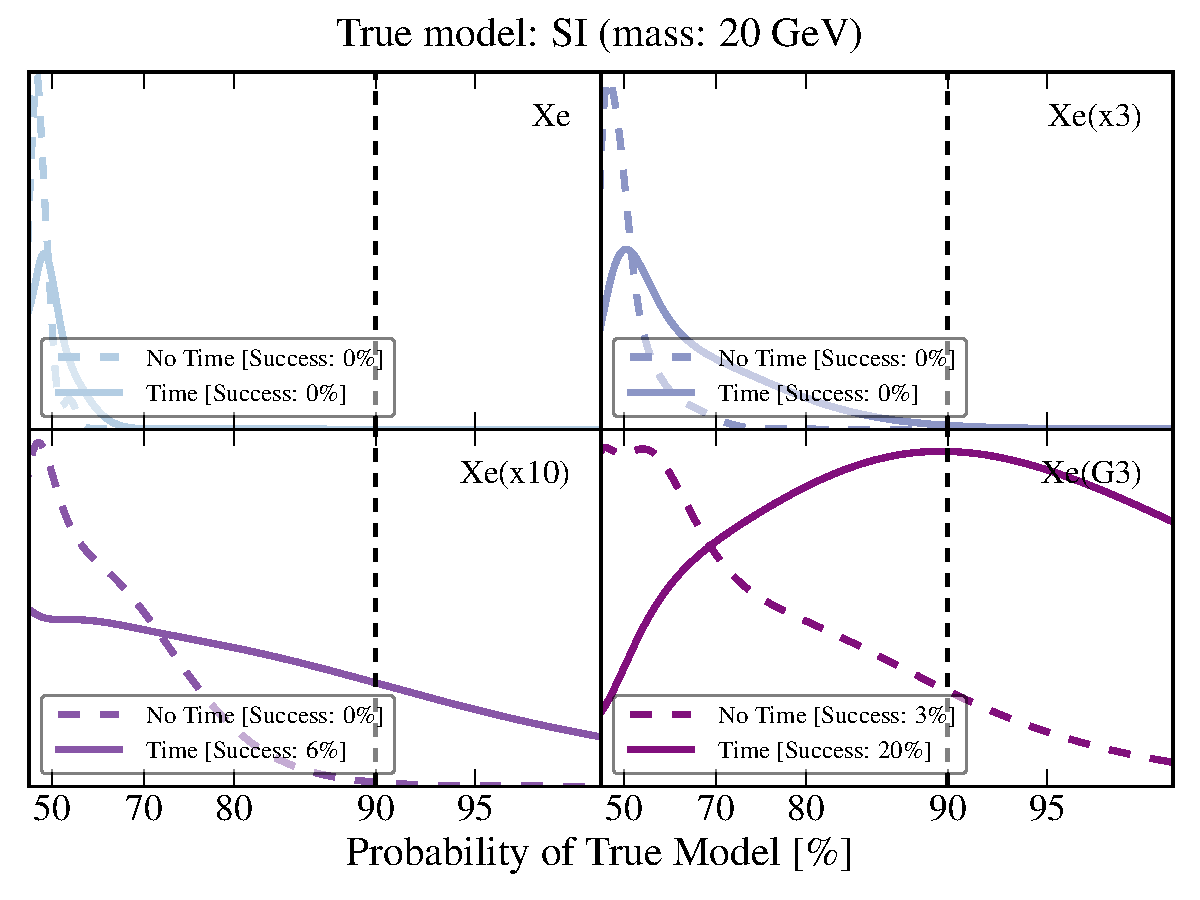
\includegraphics[width=0.7\textwidth]{plots/PDF_20GeV_SI_Higgs_50sims_Xe_Xe3x_Xe10x_XeG3_GF_TNT.pdf}
\caption{\label{fig:500gev_anapole_XeFull_TNT_GF}}
\end{figure*}

\begin{figure*}
\centering
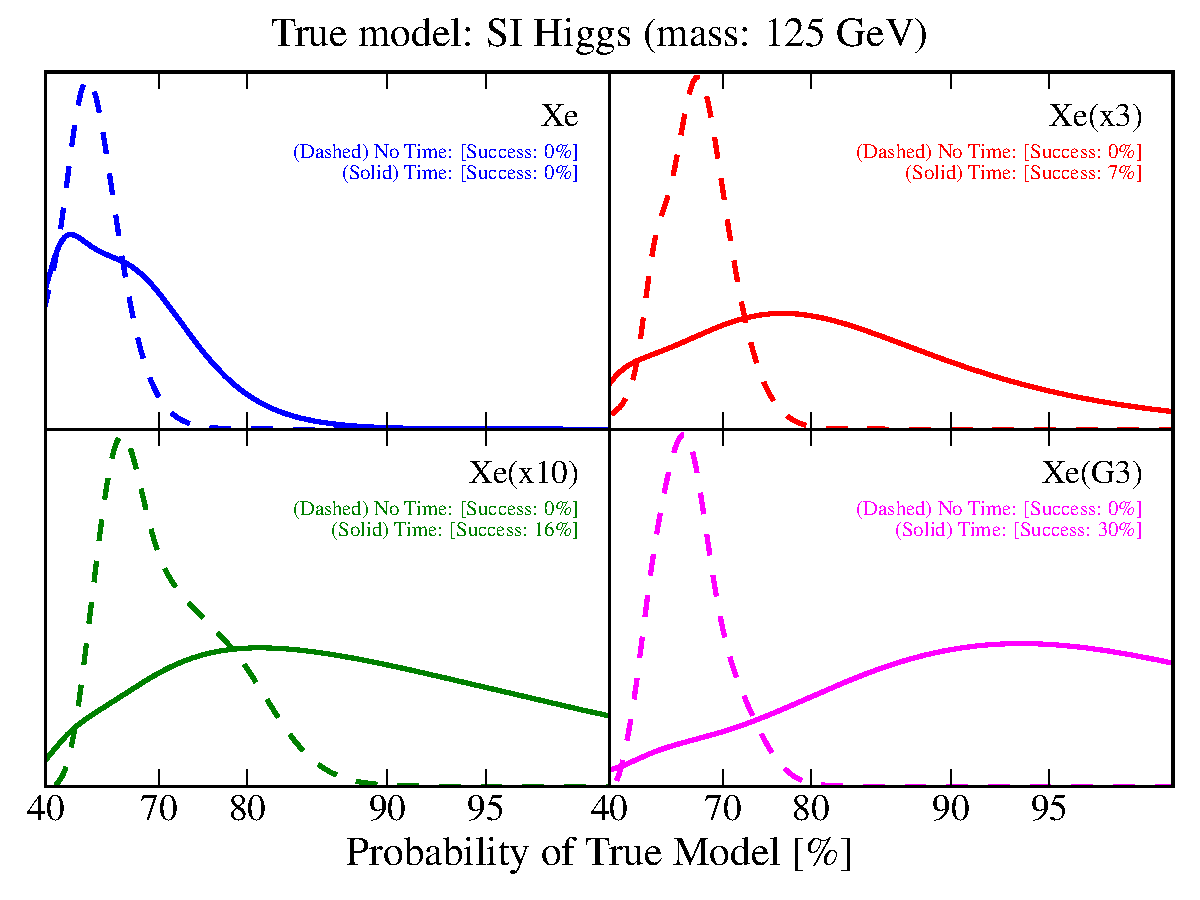
\includegraphics[width=0.7\textwidth]{plots/PDF_125GeV_SI_Higgs_50sims_Xe_Xe3x_Xe10x_XeG3_GF_TNT.pdf}
\caption{\label{fig:500gev_anapole_XeFull_TNT_GF}}
\end{figure*}

\begin{figure*}
\centering
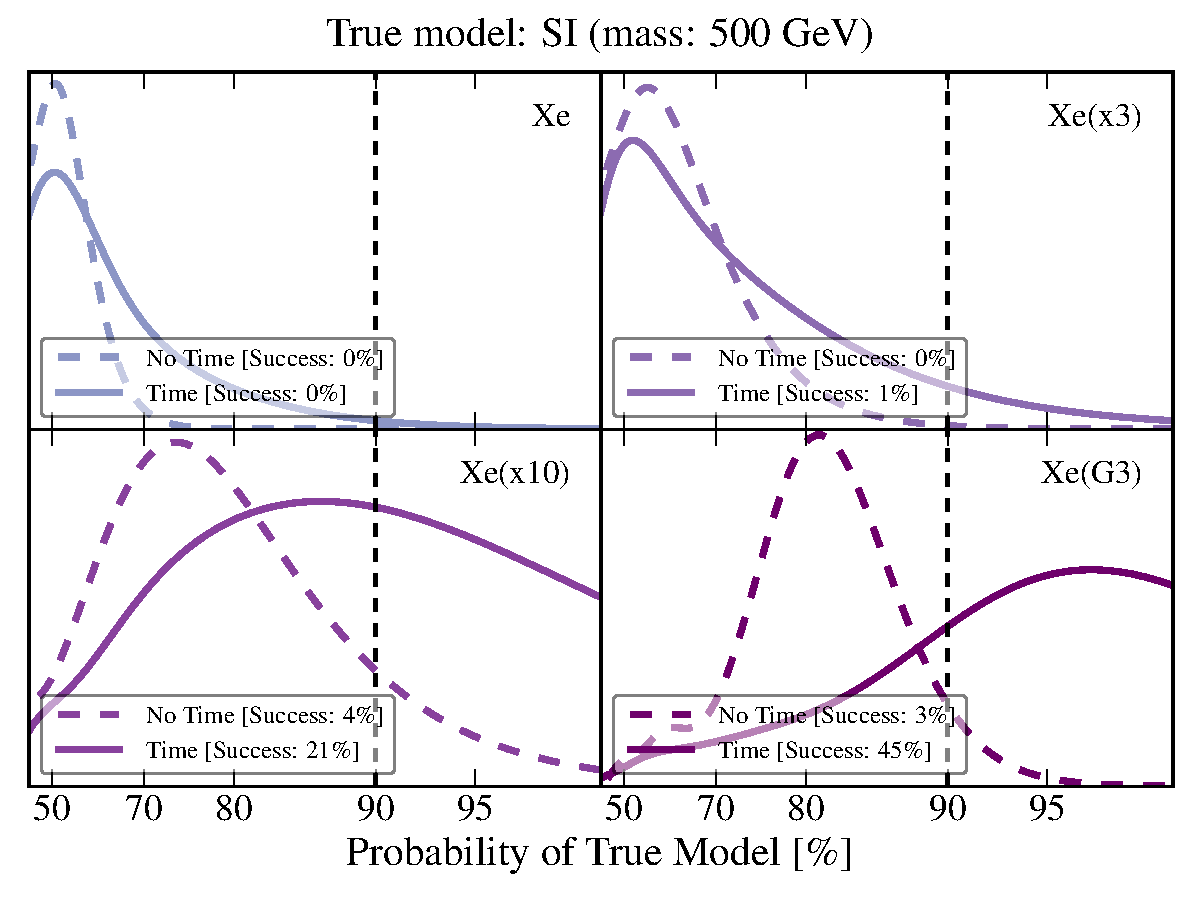
\includegraphics[width=0.7\textwidth]{plots/PDF_500GeV_SI_Higgs_50sims_Xe_Xe3x_Xe10x_XeG3_GF_TNT.pdf}
\caption{\label{fig:500gev_anapole_XeFull_TNT_GF}}
\end{figure*}





\section{Results}

\section{Conclusions}



\bibliographystyle{JHEP}
\bibliography{mod-sel}

\end{document}